\documentclass{beamer}

\usepackage[utf8]{inputenc}
\usepackage[english]{babel}
\usepackage{graphicx}
\usepackage{color}
\usepackage{natbib}
\usepackage{amssymb}
\usepackage{algorithm}
\usepackage{algpseudocode}
\usepackage{caption}
\usepackage{euler}
\usepackage{amsmath}
\usepackage{tikz}
\usetikzlibrary{arrows,calc,tikzmark,shapes.misc}

\tikzset{every picture/.style=remember picture}
% Define a TikZ node for math content:
\newcommand{\mathnode}[2]{%
  \mathord{\tikz[baseline=(#1.base), inner sep = 0pt]{\node (#1) {$#2$};}}}

\DeclareMathOperator*{\argmin}{arg\,min}
\DeclareMathOperator*{\argmax}{arg\,max}


% Beamer layout
\hypersetup{colorlinks=True, citecolor=green, linkcolor=blue}

\let\oldbibitem=\bibitem
\renewcommand{\bibitem}[2][]{\label{#2}\oldbibitem[#1]{#2}}
\let\oldcite=\cite
\renewcommand\cite[1]{\hyperlink{#1}{\oldcite{#1}}}
\let\oldcitep=\citep
\renewcommand\citep[1]{\hyperlink{#1}{\oldcitep{#1}}}
\let\oldciteauthor=\citeauthor
\renewcommand\citeauthor[1]{\hyperlink{#1}{\oldciteauthor{#1}}}

\usetheme{boxes}
\beamertemplatenavigationsymbolsempty
\setbeamertemplate{sections/subsections in toc}[circle]
\setbeamertemplate{footline}[frame number]
\setbeamertemplate{itemize items}[circle]
\setbeamertemplate{itemize subitem}[square]

% Front slide
\title{{\bf Learning to Pivot with Adversarial Networks}\\
\href{https://arxiv.org/abs/1611.01046}{arXiv:1611.01046}}
\author{{\it Gilles Louppe}, Michael Kagan, Kyle Cranmer}
\date{November 17, 2016}

\begin{document}

\begin{frame}[plain]
\titlepage
\centering
\includegraphics[height=1.5em]{nyu.jpg}
\end{frame}


% ==============================================================================

\begin{frame}

    \begin{center}
            
\includegraphics[width=0.7\textwidth]{figures/kegl.jpg}
    \end{center}

    \begin{center}
        {\it As we know, there are known knowns; there are things we know we know.
             We also know there are known unknowns; that is to say we know there
             are some things we do not know. But there are also unknown unknowns
             – the ones we don't know we don't know [...]} -- D.R.
    \end{center}
\end{frame}


\begin{frame}
    \frametitle{Systematic uncertainties -- the known unknowns in science}

    \begin{itemize}
        \item In science, the data
        generation process is often {\color{red} not uniquely specified} or known exactly, hence to the presence
        of systematic uncertainties.

        \item Data generation processes are rather formulated as a family of data generation processes
        parametrized by {\color{blue}nuisance parameters}.

        \item One of the challenges of applying machine learning to scientific
        problems is the {\color{red} need to incorporate systematics}.
    \end{itemize}

\end{frame}

\begin{frame}
    \frametitle{Problem statement}

    \begin{itemize}
        \item Let us assume a family of data generation processes $p(X, Y, Z)$ where
        \begin{itemize}
            \item $X$ are the data,
            \item $Y$ are the target labels,
            \item $Z$ are the nuisance parameters specifying systematic uncertainties.
        \end{itemize}

        \item We want to learn a regression function $f: {\cal X} \mapsto {\cal S}$ of
        parameters $\theta_f$.

        \item We want inference based on $f(X;\theta_f)$ to be {\color{red} robust}
        to the value $z \in {\cal Z}$ of the nuisance parameter -- {\it which remains unknown at test time}.

        \begin{itemize}
            \item We want a classifier that does not change with systematic variations, even though the data might.
        \end{itemize}
    \end{itemize}
\end{frame}

\begin{frame}
    \frametitle{Pivot}

    \begin{itemize}
        \item     We define robustness as requiring the distribution of $f(X;\theta_f)$
            conditional on $Z$ (and possibly $Y$) to be {\color{red}invariant with the nuisance
            parameter} $Z$.
            That is, such that
            $$p(f(X;\theta_f) = s|z) = p(f(X;\theta_f) = s|z')$$
            for all $z,z' \in {\cal Z}$ and all values $s \in {\cal S}$ of $f(X;\theta_f)$.
            If $f$ satisfies this criterion, then $f$ is known as a {\color{blue} pivotal quantity}.

        \vspace{1cm}

        \item Alternatively, this amounts to find $f$ such that $f(X;\theta_f)$ and $Z$ are {\color{red} independent random variables}.
    \end{itemize}

\end{frame}


% ==============================================================================

\begin{frame}
    \frametitle{Adversarial Networks}

    \begin{itemize}
        \item Let consider {\color{blue} a classifier $f$} built as usual, minimizing the cross-entropy
            $${\cal L}_f(\theta_f) = \mathbb{E}_{x \sim X} \mathbb{E}_{y \sim Y|x} [- \log p_{\theta_f}(y|x)].$$

        \item We pit $f$ against {\color{red} an adversary network $r$} producing
        as output a function $p_{\theta_r}(z|f(X;\theta_f)=s)$ modeling the posterior
        probability density of the nuisance parameter conditional on $f(X;\theta_f)=s$.
        We set $r$ to minimize the cross entropy
            $${\cal L}_r(\theta_f, \theta_r) = \mathbb{E}_{s \sim f(X;\theta_f)} \mathbb{E}_{z \sim Z|s}[- \log p_{\theta_r}(z|s)].$$

        \begin{itemize}
            \item If the adversary can predict the nuisance parameter from the classifier's output, then it means that some
            information about the nuisance parameter is carried out through it: the classifier is dependent on the systematics.
        \end{itemize}

    \end{itemize}
\end{frame}

\begin{frame}[fragile]
    \tikzstyle{every node}=[font=\scriptsize]
    \begin{center}
        \usetikzlibrary{arrows}
        \def\layersep{1cm}

        \begin{tikzpicture}[shorten >= 1pt, ->, node distance=\layersep,scale=0.55, every node/.style={scale=0.55}]
        \tikzstyle{neuron} = [circle, minimum size=0.25cm, draw=black!30, line width=0.3mm, fill=white]

        % Classifier f
        \node at (2,0) {Classifier $f$};
        \draw (-1,-0.5) rectangle (4,-5.5);

        \path[->, shorten >= 0pt] (-2,-3) edge (-1,-3);
        \node[left] at (-2,-3) {$X$};

        \path[-o, shorten >= 0pt] (1.5,-6.5) edge (1.5,-5.5);
        \node[below] at (1.5,-6.5) {$\theta_f$};

        \path[->, shorten >= 0pt] (3.5,-3) edge (6.5,-3);
        \node[above] at (5.25,-3) {$f(X;\theta_f)$};

        \path[dashed,-] (5.25,-3) edge (5.25,-6.5);
        \node[below] at (5.25,-6.5) {${\cal L}_f(\theta_f)$};

        \foreach \name / \y in {1,...,3}
            \node[neuron] (f-I-\name) at (-0.5,-1-\y) {};

        \foreach \name / \y in {1,...,5}
            \node[neuron] (f-H1-\name) at (-0.5cm+\layersep,-\y cm) {};
        \foreach \name / \y in {1,...,5}
            \node[neuron] (f-H2-\name) at (-0.5cm+3*\layersep,-\y cm) {};

        \node[neuron] (f-O) at (-0.5cm+4*\layersep,-3cm) {};

        \foreach \source in {1,...,3}
            \foreach \dest in {1,...,5}
                \path[black!20] (f-I-\source) edge (f-H1-\dest);

        \foreach \source in {1,...,5}
            \path[black!30] (f-H2-\source) edge (f-O);

        \node[black!30] at (1.5,-3) {...};

        % Adversary r
        \node at (11.75,0) {Adversary $r$};
        \draw (6.5,-0.5) rectangle (11.5,-5.5);

        \node[above] at (12.75,-2) {$\gamma_1(f(X;\theta_f);\theta_r)$};
        \path[-o, shorten >= 0pt] (11,-2.0) edge (14,-2.0);
        \node[above] at (12.75,-3) {$\gamma_2(f(X;\theta_f);\theta_r)$};
        \path[-o, shorten >= 0pt] (11,-3) edge (14,-3);
        \node[above] at (12.75,-4) {$\dots$};
        \path[-o, shorten >= 0pt] (11,-4) edge (14,-4);

        \path[-o, shorten >= 0pt] (9,-6.5) edge (9,-5.5);
        \node[below] at (9,-6.5) {$\theta_r$};

        \foreach \name / \y in {1,...,1}
            \node[neuron] (r-I-\name) at (7,-2-\y) {};

        \foreach \name / \y in {1,...,5}
            \node[neuron] (r-H1-\name) at (7cm+\layersep,-\y cm) {};
        \foreach \name / \y in {1,...,5}
            \node[neuron] (r-H2-\name) at (7cm+3*\layersep,-\y cm) {};

        \node[neuron] (r-O1) at (7cm+4*\layersep,-2cm) {};
        \node[neuron] (r-O2) at (7cm+4*\layersep,-3cm) {};
        \node[neuron] (r-O3) at (7cm+4*\layersep,-4cm) {};

        \foreach \source in {1,...,1}
            \foreach \dest in {1,...,5}
                \path[black!20] (r-I-\source) edge (r-H1-\dest);

        \foreach \source in {1,...,5}
            \path[black!30] (r-H2-\source) edge (r-O1);
        \foreach \source in {1,...,5}
            \path[black!30] (r-H2-\source) edge (r-O2);
        \foreach \source in {1,...,5}
            \path[black!30] (r-H2-\source) edge (r-O3);

        \node[black!30] at (9,-3) {...};

        \draw (14,-1.5) rectangle (17,-4.5);
        \path[->, shorten >= 0pt] (15.5,-0.5) edge (15.5,-1.5);
        \node[above] at (15.5,-0.5) {$Z$};
        \path[->, shorten >= 0pt] (15.5,-4.5) edge (15.5,-5.5);
        \node[below] at (15.5,-5.5) {$p_{\theta_r}(Z|f(X;\theta_f))$};
        \node at (15.5,-3) {${\cal P}(\gamma_1, \gamma_2, \dots)$};

        \draw[dashed,-] (15.5,-5) -| (12.75,-6.5);
        \node[below] at (12.75,-6.5) {${\cal L}_r(\theta_f, \theta_r)$};

        \end{tikzpicture}
    \end{center}
\end{frame}

\begin{frame}
    \frametitle{$Z$ can be either categorical or continuous}

    \begin{columns}
        \begin{column}{0.6\textwidth}
            \begin{itemize}
                \item If $Z$ is {\color{blue} categorical}, then the posterior can be modeled with a standard (probabilistic) classifier.

                \vspace{1cm}

                \item If $Z$ is {\color{red} continuous}, then the posterior can be modeled with a {\it mixture density network}.

                \vspace{1cm}

                \item No constraint on the prior $p(Z)$.
            \end{itemize}
        \end{column}
        \begin{column}{0.5\textwidth}
            \begin{center}
                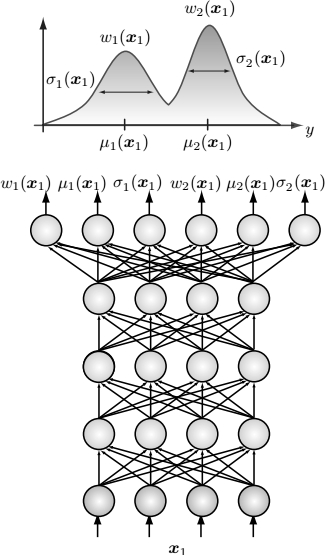
\includegraphics[width=0.8\textwidth]{figures/mdn.jpg}\\
                {\it Mixture density network}
            \end{center}
        \end{column}
    \end{columns}
\end{frame}


% ==============================================================================

\begin{frame}
    \frametitle{Adversarial training}

    \begin{columns}
        \begin{column}{0.7\textwidth}
            {\it
            What if the classifier forces the adversary to perform worse by simultaneously maximizing ${\cal L}_r$?
            It should reduce its dependence on the nuisance parameter, shouldn't it?}
        \end{column}
        \begin{column}{0.3\textwidth}
            \begin{center}
                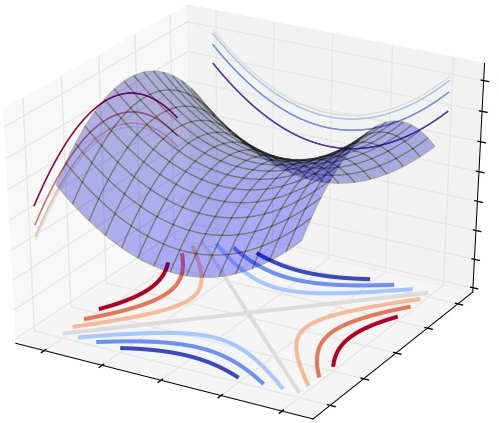
\includegraphics[width=\textwidth]{figures/saddle.jpg}
            \end{center}
        \end{column}
    \end{columns}

    \vspace{0.5cm}

    Formally, let us consider the value function
    $$E(\theta_f, \theta_r) = {\cal L}_f(\theta_f) - {\cal L}_r(\theta_f, \theta_r)$$
    that we optimize by finding the minimax solution
    $$\hat\theta_f, \hat\theta_r = \arg \min_{\theta_f} \max_{\theta_r} E(\theta_f, \theta_r).$$

\end{frame}

\begin{frame}
    \frametitle{Theoretical motivation}

    {\bf Proposition.}
    {\it If there exists a minimax solution $(\smash{\hat\theta}_f, \smash{\hat\theta}_r)$
    such that
    $E(\hat\theta_f, \hat\theta_r) = H({Y|X}) - H(Z)$, then
    $f(\cdot;\smash{\hat\theta}_f)$ is both an optimal classifier and a pivotal
    quantity.}

    \vspace{0.5cm}

    Proof (sketch):
    {\scriptsize
    \begin{align*}
         & \min_{\theta_f} \max_{\theta_r} {\cal L}_f(\theta_f) - {\cal L}_r(\theta_f, \theta_r) \\
         =& \min_{\theta_f} {\cal L}_f(\theta_f) - \mathbb{E}_{s \sim f(X;\theta_f)} [H(Z|f(X;\theta_f) = s)] \\
         =& \min_{\theta_f} {\cal L}_f(\theta_f) - H(Z|f(X;\theta_f)) \\
         \geq& H({Y|X}) - H(Z)
    \end{align*}}
    where the equality holds when
    \begin{itemize}
        \item  $f$ is an optimal classifier (in which case ${\cal L}_f(\theta_f) = H({Y|X})$);
        \item  $f(X;\theta_f)$ and $Z$ are independent random variables (in which case $H(Z|f(X;\theta_f)) = H(Z)$).
    \end{itemize}
\end{frame}


\begin{frame}[fragile]
    \frametitle{Alternating stochastic gradient descent}
        \begin{minipage}{\linewidth}
            \scriptsize

        \begin{algorithmic}[1]
            \For{$t=1$ to $T$}
                \For{$k=1$ to $K$} \Comment{Update $r$}
                    \State{Sample minibatch $\{x_m, z_m, s_m = f(x_m;\theta_f) \}_{m=1}^M$} of size $M$;
                    \State{With $\theta_f$ fixed, update $r$ by ascending its stochastic gradient $\nabla_{\theta_r} E(\theta_f, \theta_r) :=$
                    $$\nabla_{\theta_r} \sum_{m=1}^M \log p_{\theta_r}(z_m|s_m)  ;$$}
                \EndFor
                \State{Sample minibatch $\{x_m, y_m, z_m, s_m = f(x_m;\theta_f)  \}_{m=1}^M$} of size $M$; \Comment{Update $f$}
                \State{With $\theta_r$ fixed, update $f$ by descending its stochastic gradient $\nabla_{\theta_f} E(\theta_f, \theta_r) :=$
                $$\nabla_{\theta_f}  \sum_{m=1}^M \left[ -\log p_{\theta_f}(y_m|x_m)  +\log p_{\theta_r}(z_m|s_m)  \right],$$
                \indent where $p_{\theta_f}(y_m|x_m)$ denotes $\mathbf{1}(y_m=0)(1-s_m) + \mathbf{1}(y_m=1)s_m$;}
            \EndFor
        \end{algorithmic}

        \end{minipage}
\end{frame}


\begin{frame}
    \frametitle{Accuracy versus robustness trade-off}

    \begin{itemize}
        \item The assumption of existence of a classifier that is both optimal and pivotal may not hold.

              \vspace{0.5cm}

        \item However, the value function $E$ can be rewritten as
            $$E_\lambda(\theta_f, \theta_r) = {\cal L}_f(\theta_f) - \lambda {\cal L}_r(\theta_f, \theta_r)$$
            where $\lambda$ is a hyper-parameter controlling the trade-off between
            the performance of $f$ and its independence with respect to the nuisance
            parameter.

        \begin{itemize}
            \item Setting $\lambda$ to a large value enforces $f$ to be pivotal.
            \item Setting $\lambda$ close to $0$ constraints $f$ to be optimal.
        \end{itemize}
    \end{itemize}
\end{frame}



% ==============================================================================

\begin{frame}
    \frametitle{Toy example}

    \begin{columns}[t]
        \begin{column}{0.8\textwidth}
            \begin{itemize}
                \item Binary classification of 2D
               data drawn from multivariate gaussians with equal priors, such that
               {\scriptsize
               \begin{align*}
                   x &\sim {\cal N}\left ((0,0), \begin{bmatrix}
                                             1 & -0.5 \\
                                             -0.5 & 1
                                           \end{bmatrix}\right) &\text{ when } Y=0, \\
                   x &\sim {\cal N}\left ((1,1+Z),  \begin{bmatrix}
                                             1 & 0 \\
                                             0 & 1
                                            \end{bmatrix}\right) &\text{ when } Y=1.
               \end{align*}}
               \item The continuous nuisance parameter $Z$ represents in this case our
               uncertainty about the exact location of the mean of the second gaussian.
               We assume a gaussian prior $z \sim {\cal N}(0,1)$.

               \item We assume training data $\{ x_i, y_i, z_i \}_{i=1}^N \sim p(X,Y,Z)$.
            \end{itemize}
        \end{column}
        \begin{column}{0.3\textwidth}
            \begin{center}
                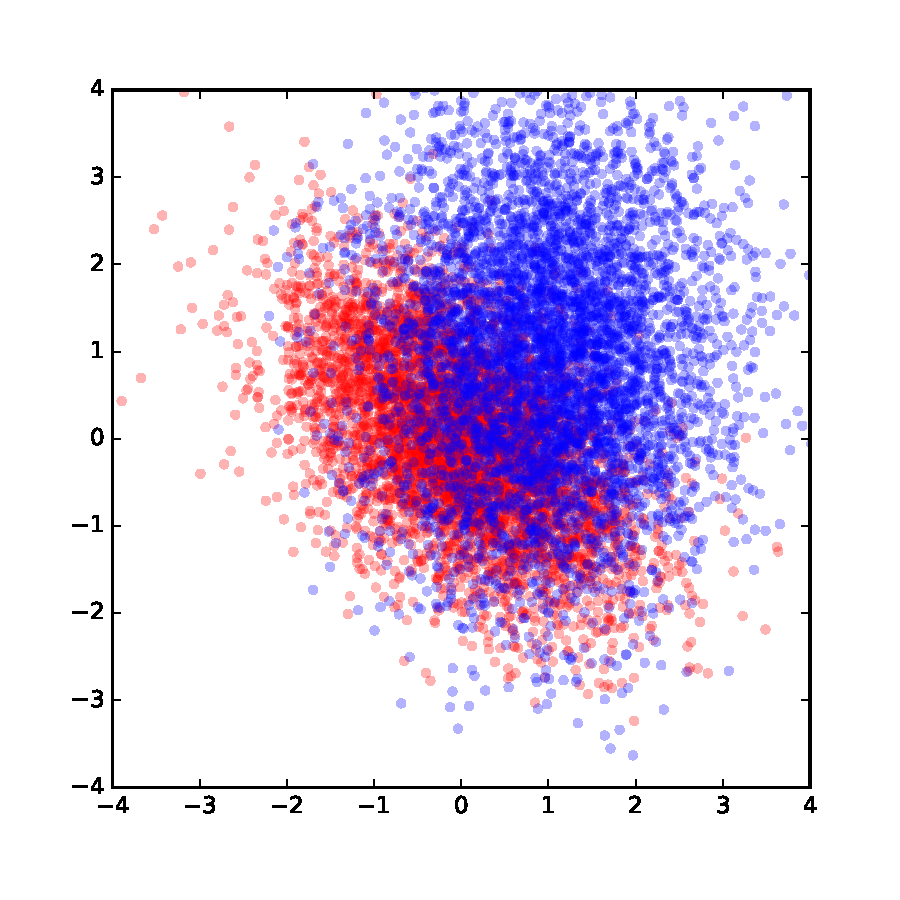
\includegraphics[width=\textwidth]{figures/toy-data.pdf}
            \end{center}
        \end{column}
    \end{columns}
\end{frame}


\begin{frame}
    \frametitle{Standard training without the adversary $r$}

    \begin{center}
        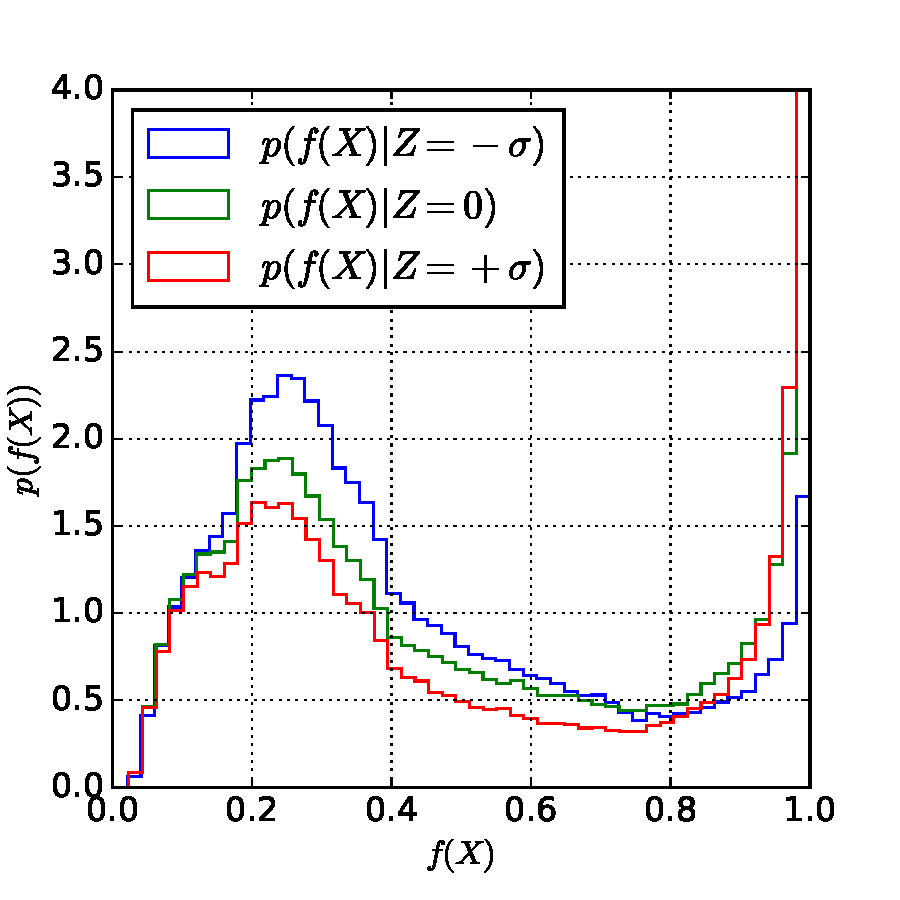
\includegraphics[width=0.48\textwidth]{figures/f-plain.pdf}
        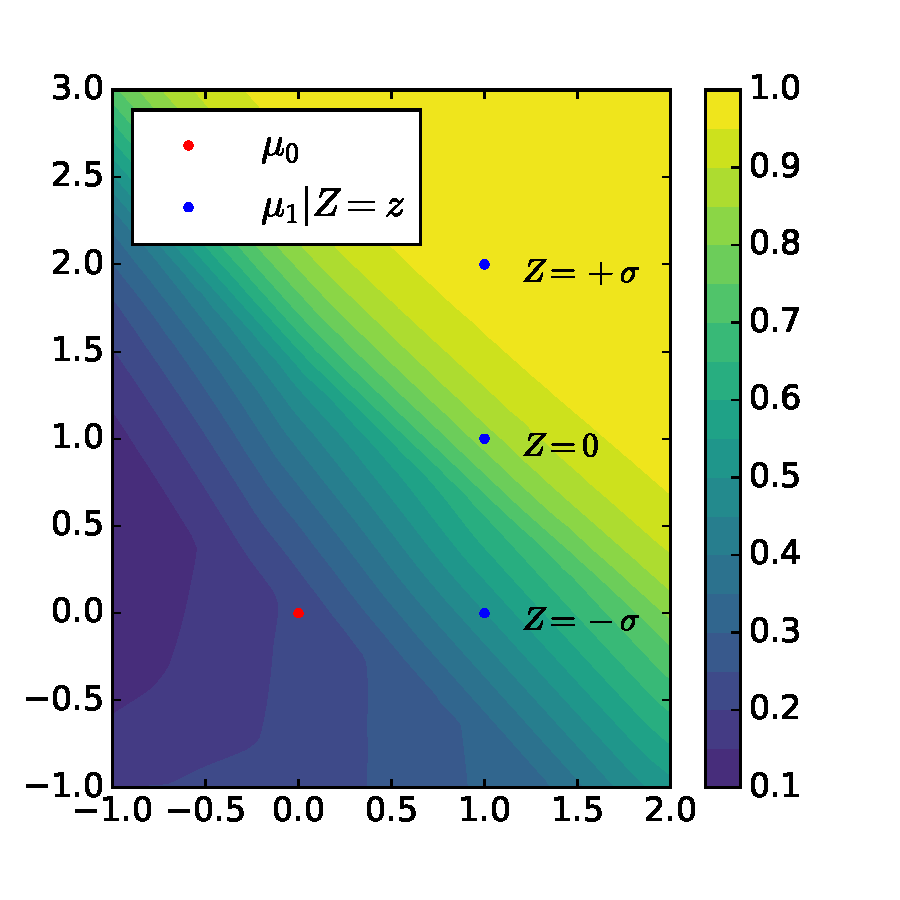
\includegraphics[width=0.48\textwidth]{figures/surface-plain.pdf}\\
        (Left) The conditional probability distributions \\
        of $f(X;\theta_f)|Z=z$ {\color{red}changes with $z$}.

        \vspace{0.25cm}

        (Right) The decision surface {\color{red} strongly depends on $X_2$}.
    \end{center}
\end{frame}


\begin{frame}
    \frametitle{Reshaping $f$ with adversarial training}

    \begin{center}
        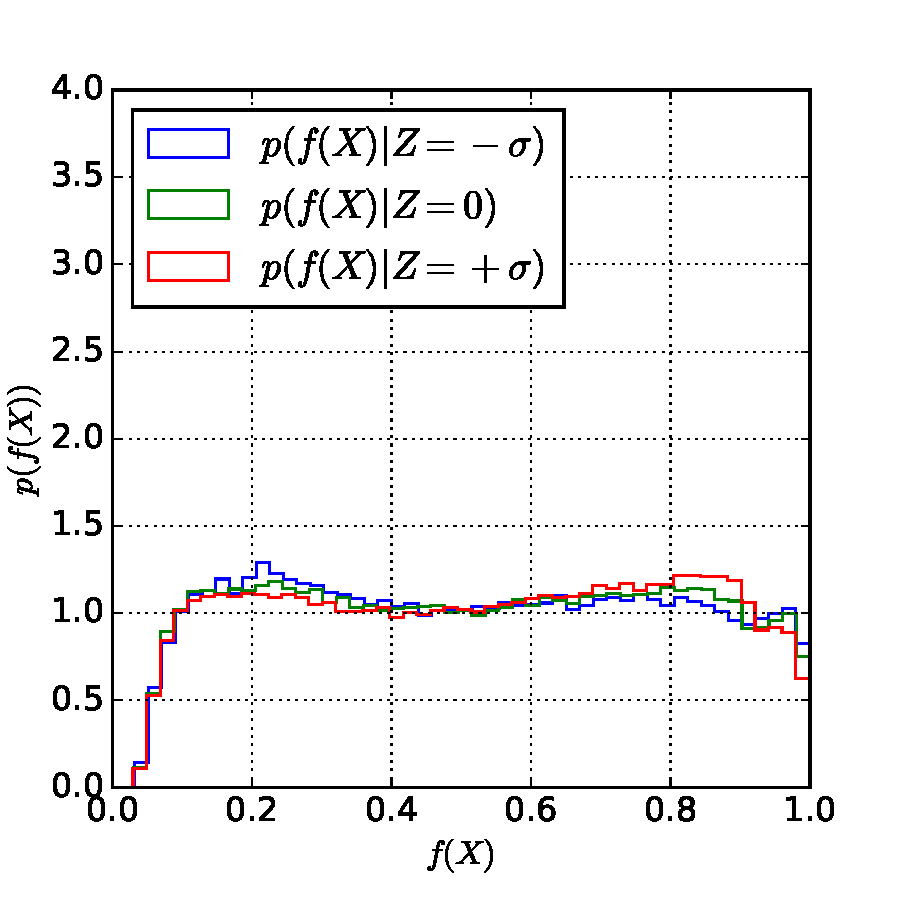
\includegraphics[width=0.48\textwidth]{figures/f-adversary.pdf}
        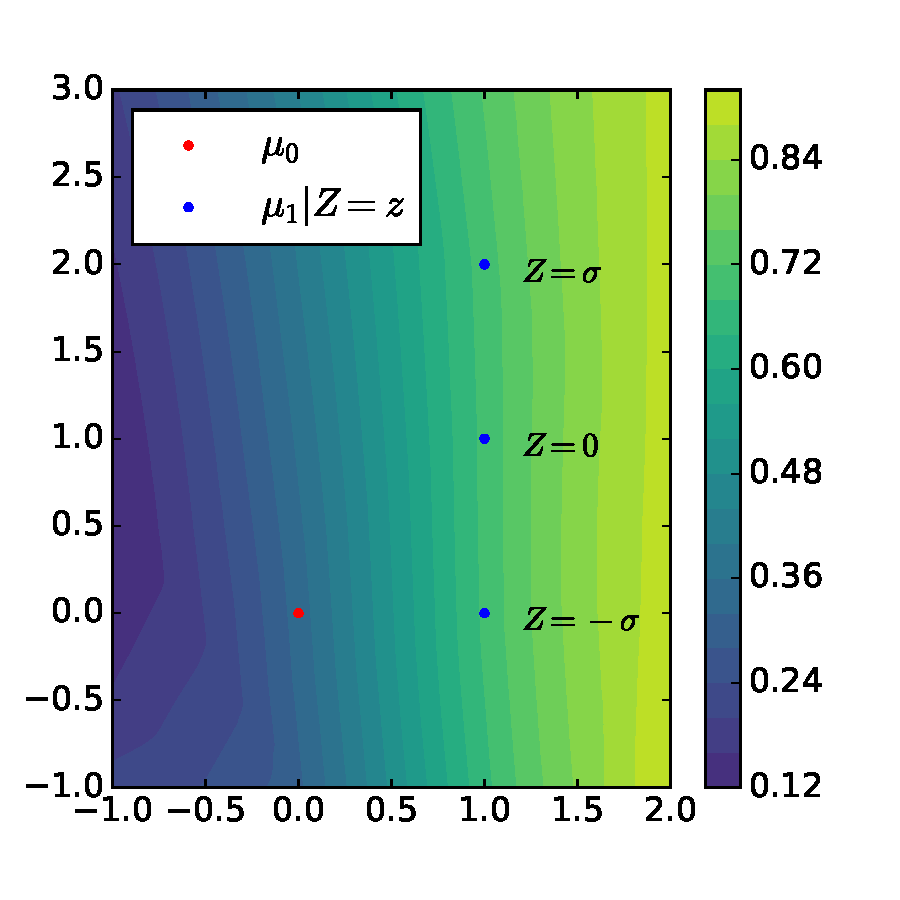
\includegraphics[width=0.48\textwidth]{figures/surface-adversary.pdf}\\
        (Left) The conditional probability distributions \\
        of $f(X;\theta_f)|Z=z$ are {\color{blue}now (almost) invariant with $z$}!

        \vspace{0.25cm}

        (Right) The decision surface is {\color{blue} now independent of $X_2$}.
    \end{center}
\end{frame}

\begin{frame}
    \frametitle{Dynamics of adversarial training}

    \begin{center}
        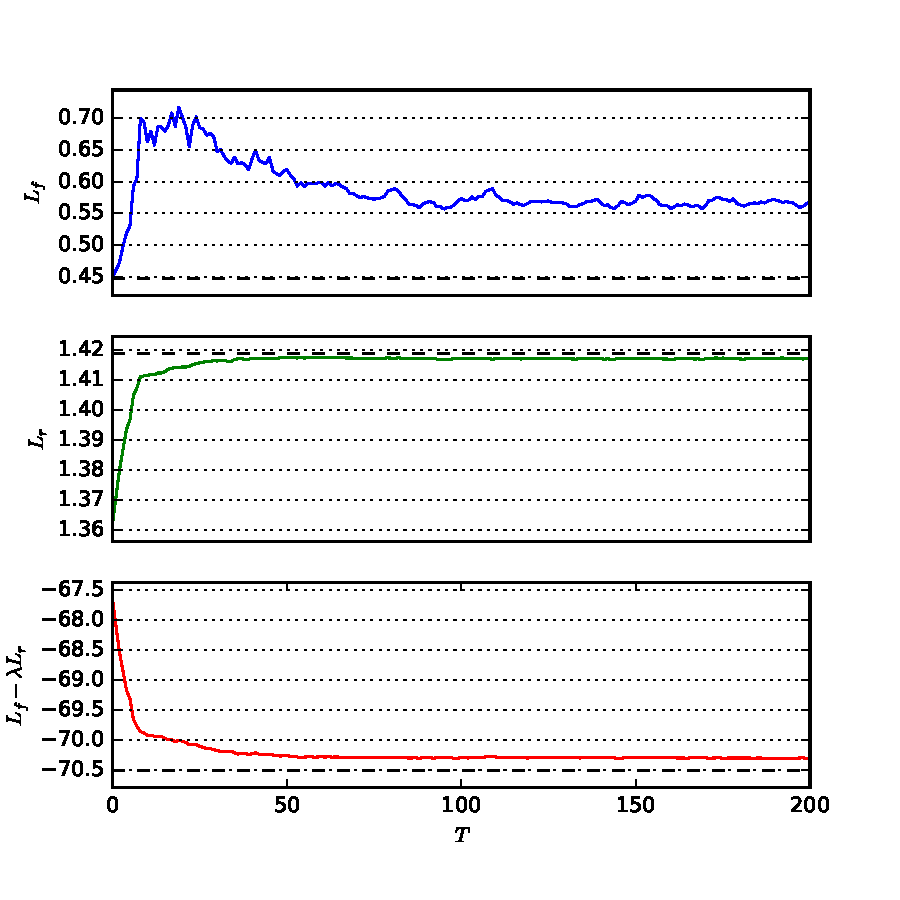
\includegraphics[width=0.8\textwidth]{figures/training.pdf}
    \end{center}
\end{frame}


% ==============================================================================

\begin{frame}
    \frametitle{High energy physics example}


    \begin{columns}[t]
        \begin{column}{0.6\textwidth}
            \begin{itemize}
                \item Discriminate between QCD jets ($Y=0$) and $W$-jets ($Y=1$)
                from high-level features (data from Baldi et al, \href{http://arxiv.org/abs/1603.09349}{arXiv:1603.09349}).

                \vspace{0.5cm}

                \item Taking some liberty, we consider an extreme categorical nuisance parameter where
                \begin{itemize}
                    \item $Z=0$ corresponds to events without pileup,
                    \item $Z=1$ corresponds to events with pileup, for which there are
                    an average of 50 independent pileup interactions overlaid.
                \end{itemize}
            \end{itemize}
        \end{column}
        \begin{column}{0.45\textwidth}
            \begin{center}
                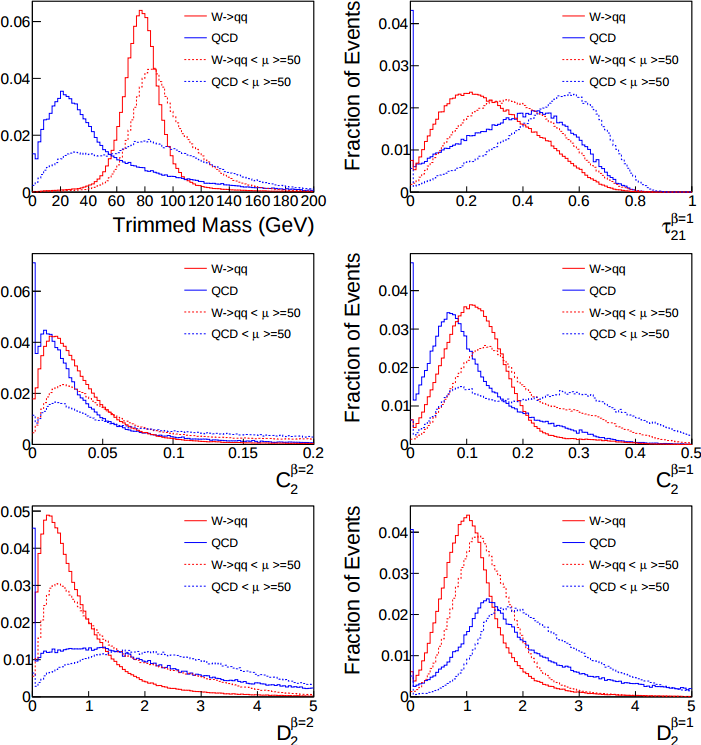
\includegraphics[width=\textwidth]{figures/jets.png}
            \end{center}
        \end{column}
    \end{columns}



\end{frame}


\begin{frame}
    \frametitle{Maximizing significance by tuning $\lambda$}

    \begin{itemize}
        \item Since we do not expect to find a classifier $f$ that is both optimal and pivotal,
              we optimize the accuracy-independence trade-off by {\color{blue} tuning $\lambda$ with respect
        to a higher level objective}.

        \item Cut and count analysis: A natural higher-level context is a hypothesis test of
        a null with no signal events against an alternate hypothesis that is a mixture
        of signal and background events.
        \begin{itemize}
            \item Background = 1000 weighted QCD jets, Signal = 100 weighted boosted W's.
            \item Without systematics, optimizing ${\cal L}_f$
            indirectly optimizes the power of a classical hypothesis test.
            \item With systematics, we need to balance classification performance
            against robustness to the nuisance parameter.
            \item To this end, we use the {\color{red}Approximate Median Significance (AMS)} as higher-level objective.
            \item Note that since we are performing a hypothesis test of
            the null, we only wish to impose the pivotal property on background events.
        \end{itemize}

    \end{itemize}
\end{frame}

\begin{frame}
    \begin{center}
        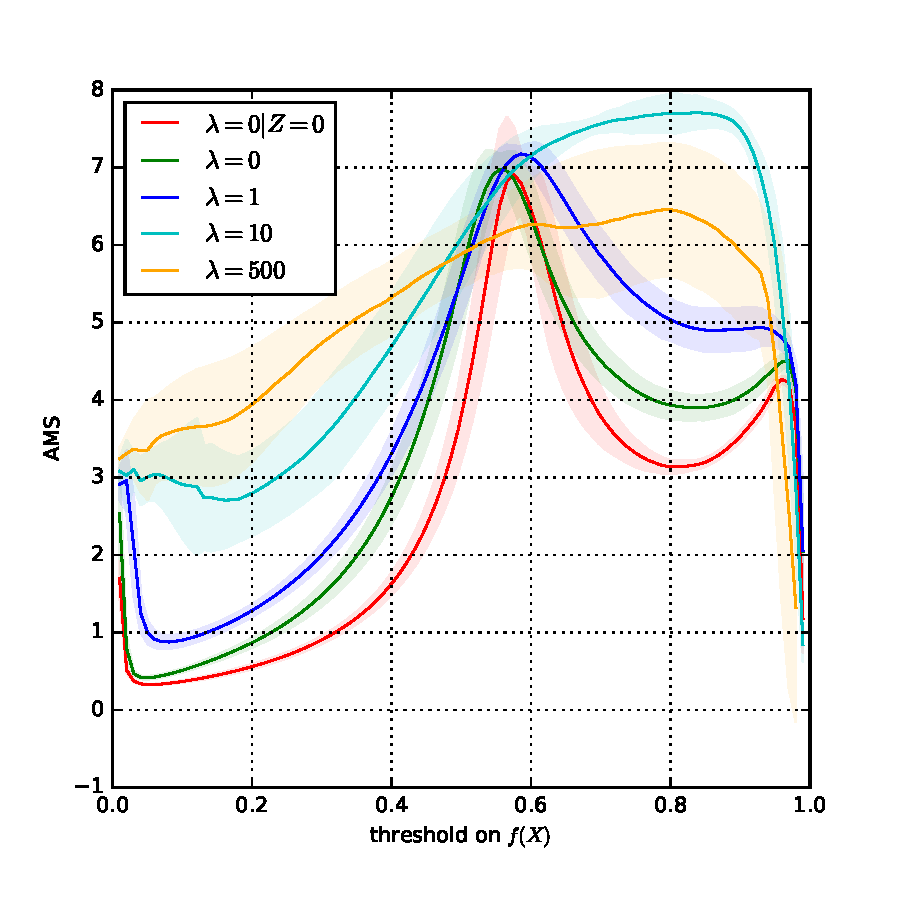
\includegraphics[width=0.6\textwidth]{figures/ams.pdf}
    \end{center}

        {\color{red}$\lambda=0|Z=0$}: standard training from $p(X, Y, Z=0)$.\\
        {\color{green}$\lambda=0$}: standard training from $p(X, Y, Z)$.\\
        {\color{cyan}$\lambda=10$}: trading
         accuracy for robustness wrt pileup
        results in a net benefit in terms of maximum statistical significance.
\end{frame}


% ==============================================================================

\begin{frame}
    \frametitle{Summary}

    \begin{itemize}
        \item We proposed a principled approach based on adversarial networks
        for building a model
        whose output can be constrained to be independent of a chosen
        nuisance parameter (or any random variable).

        \item The method supports both categorical and continuous
        nuisance parameters.

        \item Control is offered to tune the accuracy versus robustness trade-off in
        order to maximize a higher-level objective.

        \vspace{1cm}

        \item {\color{red} We are looking for opportunities of (real) physics use cases! Come talk to us if interested!}

    \end{itemize}
\end{frame}



\end{document}
